\documentclass[a4paper]{article}
\usepackage[english]{babel}
\usepackage[utf8]{inputenc}
\usepackage{graphicx}

\title{A News System Implementation \\ C++ Programming, EDA031}

\author{Erik Hedblom, [tpi11ehe]
\and Tobias Landelius, [ael10tla]
\and Oskar Jermakowicz, [dat12oje]
\and Martin Larsson, [dat12mla]}



\date{\today}


\begin{document}
\maketitle

\newpage
\renewcommand{\contentsname}{Table of contents}
\tableofcontents
\newpage

\section{System description}
The application is a simple implementation of a news system where newsgroups and articles are stored on a server which communicates with clients that connect to it. The client is a Command Line Interface where users can execute commands to receive, edit or delete data on the server.

The implementation is divided into three packages as can be seen in Figure~\ref{fig:uml} below; \texttt{client}, \texttt{library} and \texttt{server}.

\begin{figure}[h]
    \centering
    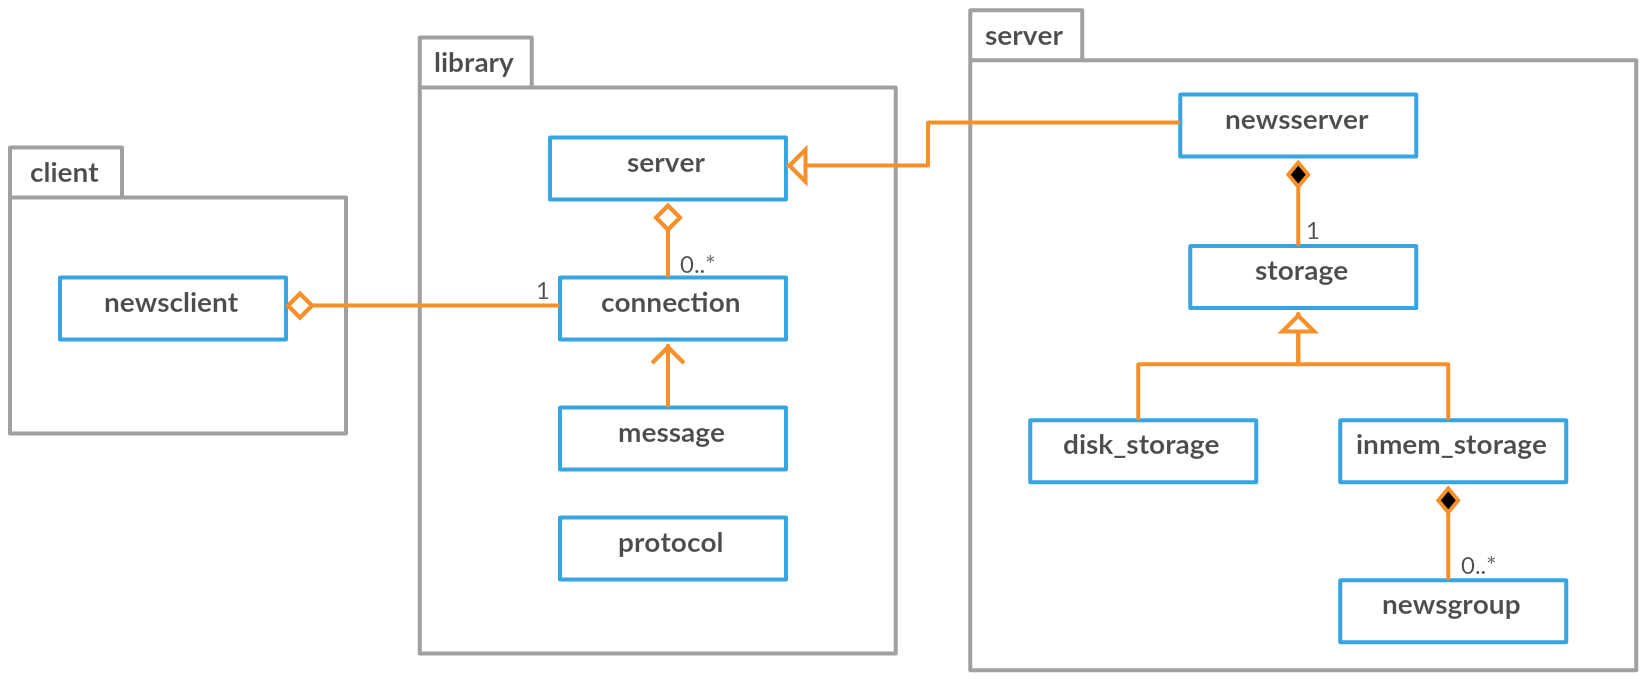
\includegraphics[width=1.0\textwidth]{uml_diagram.png}
    \caption{UML diagram of the system.}
    \label{fig:uml}
\end{figure}

The purpose of the library package is to simply handle the interaction between the server and the client. During the execution of commands on the server a given protocol is used for the communication which is defined in \texttt{protocol.h} in the library package. The purpose of both the server and the client will be further explained in detail in section~\ref{subsec:server} and \ref{subsec:client} of this report. In Appendix A an example sequence diagram can be seen, this shows the client and server interaction steps that are taken during the removal of a newsgroup when such a request comes from the client.

\subsection{Server}
\label{subsec:server}
The provided classes \texttt{Connection} and \texttt{Server} manages the actual network sockets and connected clients. From them we receive a stream of bytes to decode as commands from the clients. The decoding and execution of commands is done by \texttt{Newsserver} using the utility functions in \texttt{message}. The commands may result in changes in the database which is used to store all newsgroups and articles. There is source code for two types of databases: one only using the primary memory (\texttt{inmem\_storage} and \texttt{newsgroup}) and one working against the disk (\texttt{disk\_storage}). Both of these classses inherit from the base class \texttt{storage} making it easy to swap between the two, although \texttt{disk\_storage} is the one currently used. There is also a set of possible exceptions defined in \texttt{storage\_exception} that can happen when interacting with the database.


\subsection{Client}
\label{subsec:client}
In order to start a client, one has to run the following command on the command line in the directory of newsclient; \texttt{newsclient host-name port-number}. If the connection is successful, this will establish a connection with the server. The establishment of the connection is handled by the \texttt{NewsClient} constructor which creates a \texttt{Connection} object which will be used to communicate with the server.

Once a connection is established the \texttt{run()} method of \texttt{NewsClient} is run, and the user can now execute commands. All possible commands are explained if the user runs the command \texttt{help}, the printout of the \texttt{help} command can be seen in Appendix B.

The client parses each user input through regex to see whether the input is a valid command. This is done through \texttt{parse\_line(string)} which matches any valid commands and parameters and stores them in a vector. This vector is thereafter compared with the available commands in \texttt{handle\_command(string)}, and if it turns out the commands is valid, the corresponding method for that particular command is run in \texttt{NewsClient}. These methods simply call the different send commands in the \texttt{message} class in the \texttt{library} package. The start and end of the command is sent with the \texttt{send\_code(Connection, int)} method in \texttt{message}, where the int is the corresponding protocol definition from \texttt{protocol.h}. If the command has any parameters, these are sent with either \texttt{send\_int\_parameter(Connection, int)} or \texttt{send\_string\_parameter(Connection, string)}. Once the whole command has been sent to the server, the same method will check the servers response with \texttt{consume\_code(Connection, int)} (where int is a protocol definition) and \texttt{recv\_code(Connection)} in \texttt{message} and print the servers response to the user.


\section{Conclusion}
We fulfilled all requirements given to the extent that is possible. For example, the requirement that there should be no limitation on the number of newsgroups or articles is not realizeable. The newsserver is not particulary safe in the sense that anyone can connect to a server and modify the database. A better solution would involve users logging in and have restricted access to perhaps only read articles or only be able to delete articles created by the user.

While the disk database does work as intended it does not handle all possible errors that can arise when working against disk (files can go missing, corrupted files, permissions, etc). We did not implement all this error handling as it felt out of scope for the project.

The project as a whole felt small for the course, though, perhaps because we were a full team of four students. It would have been interesting to explore more obscure parts of C++ as there were plenty of time to complete the project.

\newpage
\section*{Appendix A}
\addcontentsline{toc}{section}{Appendix A}


\begin{figure}[!h]
    \centering
    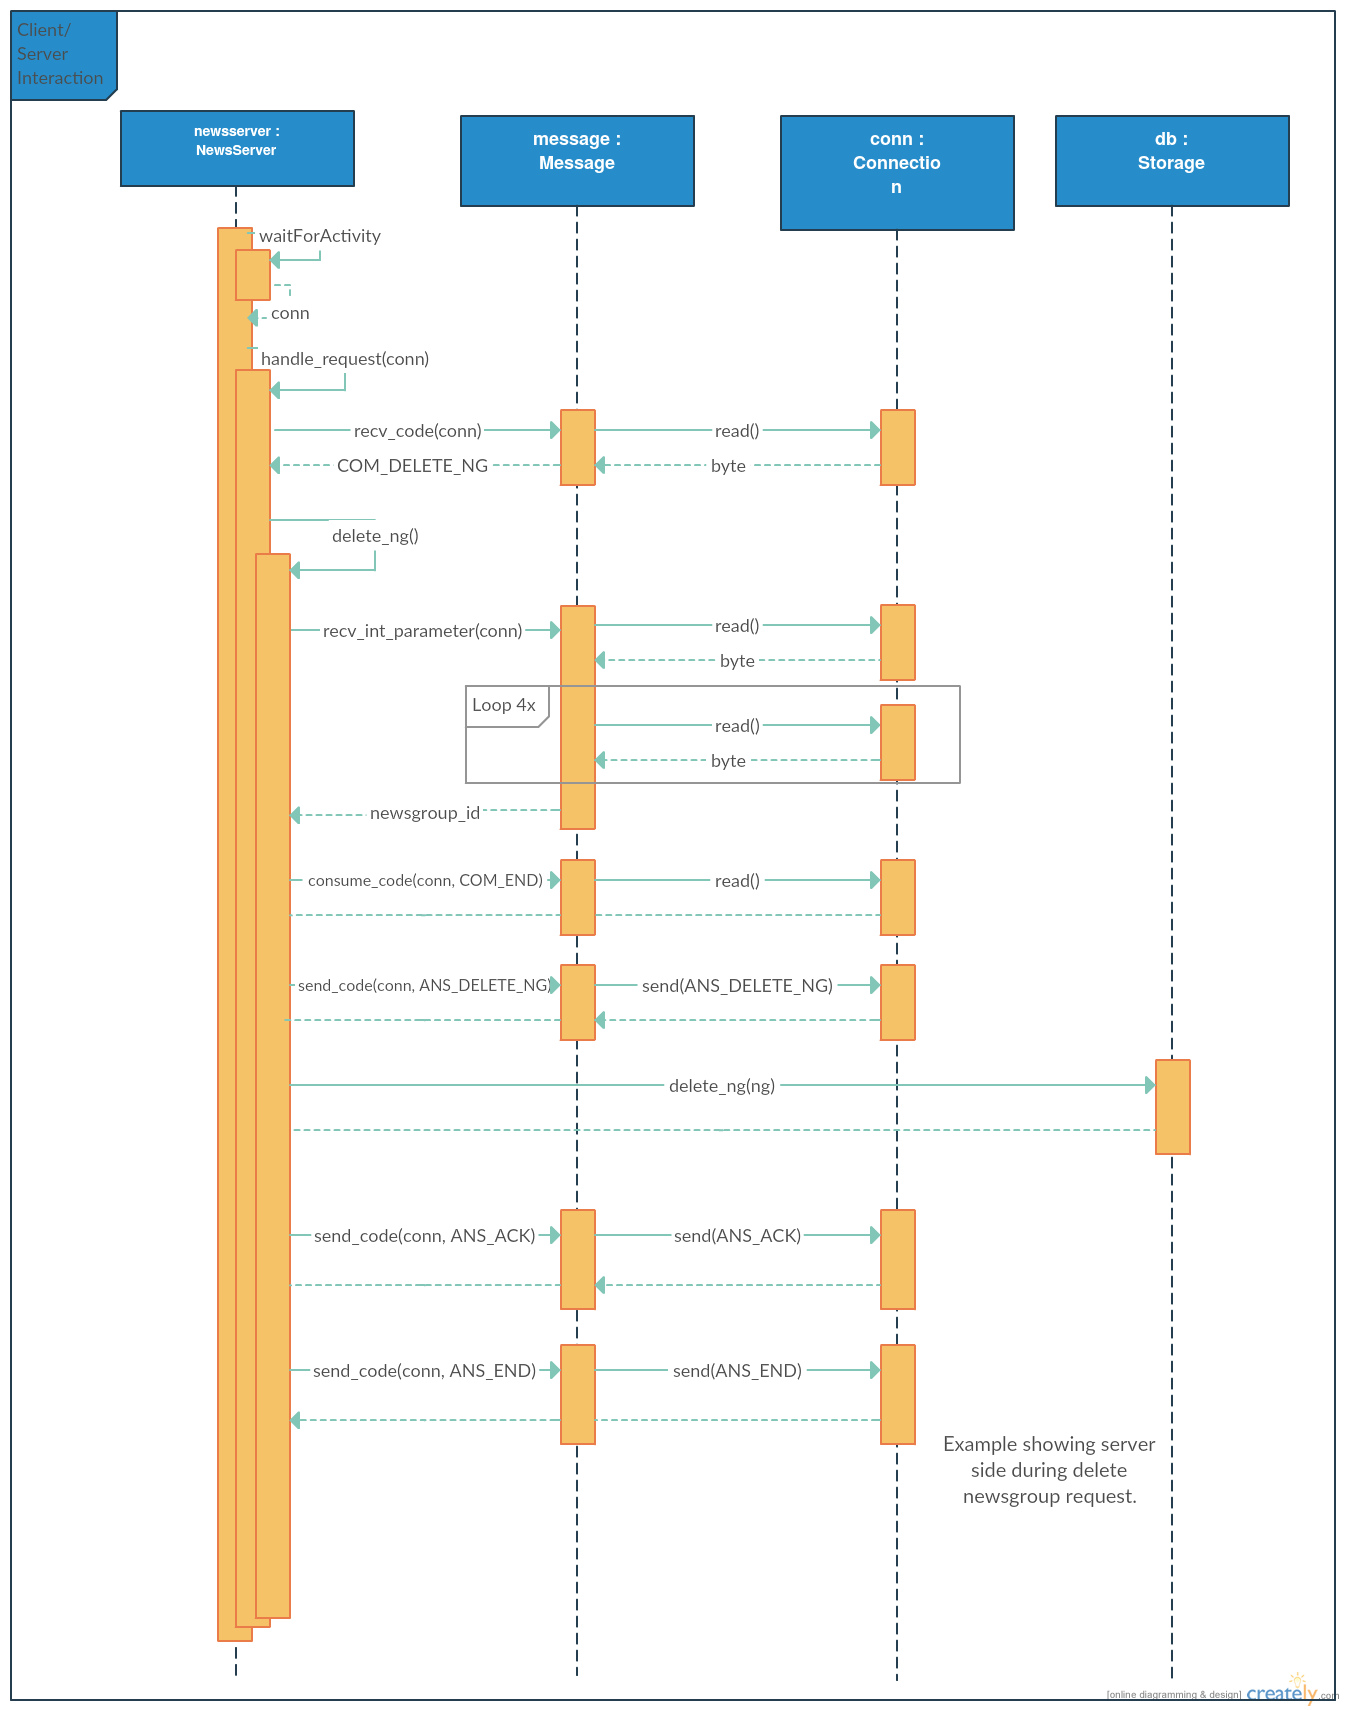
\includegraphics[width=1.1\textwidth]{sequence_uml3.png}
    \caption{The interaction between server and client.}
    \label{fig:sequence}
\end{figure}

\newpage
\section*{Appendix B}
\addcontentsline{toc}{section}{Appendix B}


\begin{figure}[h]
    \centering
    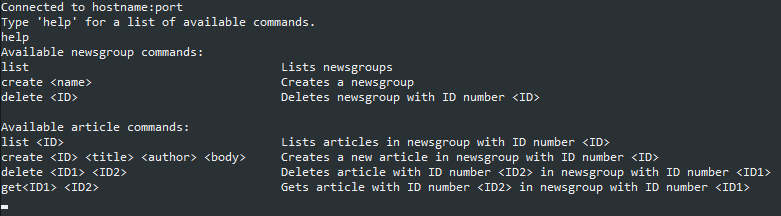
\includegraphics[width=0.9\textwidth]{help_text_appendix.png}
    \caption{Available commands, shown when the \texttt{help} command is run.}
    \label{fig:help}
\end{figure}



\end{document}
